%File: SupplementaryMaterial2027.tex
\documentclass[letterpaper]{article} % DO NOT CHANGE THIS
\usepackage[submission]{aaai2027}  % DO NOT CHANGE THIS
% The serif, sans-serif, and monospaced fonts are loaded automatically by
% aaai2027.sty (newtxtext, helvet, courier). DO NOT add font packages.
\usepackage[hyphens]{url}  % DO NOT CHANGE THIS
\usepackage{graphicx} % DO NOT CHANGE THIS
\urlstyle{rm} % DO NOT CHANGE THIS
\def\UrlFont{\rm}  % DO NOT CHANGE THIS
\usepackage{natbib}  % DO NOT CHANGE THIS AND DO NOT ADD ANY OPTIONS TO IT
\usepackage{caption} % DO NOT CHANGE THIS AND DO NOT ADD ANY OPTIONS TO IT
\usepackage{amsmath}
\usepackage{amssymb}
\usepackage{multirow}
\usepackage{booktabs}
\usepackage{fancybox}
\newcommand{\thickhline}{\noalign{\hrule height 0.8pt}}
\newcommand{\placeholder}[1]{\texttt{\{#1\}}}
\newsavebox{\promptboxcontent}
\newsavebox{\algboxcontent}
\newcounter{algorithm}
\renewcommand{\thealgorithm}{\arabic{algorithm}}
\newcommand{\algindent}{\hspace*{1.5em}}
\newcommand{\algindenttwo}{\hspace*{3em}}
\newcommand{\algindentthree}{\hspace*{4.5em}}
\newcommand{\algindentfour}{\hspace*{6em}}
\newenvironment{algbox}[1]{%
  \refstepcounter{algorithm}%
  \par\smallskip\noindent
  \begin{lrbox}{\algboxcontent}%
  \begin{minipage}{0.96\columnwidth}\small
  \hrule height 0.8pt\relax
  \vspace{2pt}\noindent\textbf{Algorithm \thealgorithm} #1\par
  \vspace{2pt}\hrule height 0.4pt\relax
  \smallskip
}{%
  \par\vspace{2pt}\hrule height 0.8pt\relax
  \end{minipage}%
  \end{lrbox}%
  \usebox{\algboxcontent}\par\smallskip
}
\newenvironment{promptbox}[1]{%
  \par\smallskip\noindent
  \textbf{#1}\par\noindent
  \setlength{\fboxsep}{6pt}%
  \setlength{\fboxrule}{0.7pt}%
  \cornersize{0.08}%
  \begin{lrbox}{\promptboxcontent}%
  \begin{minipage}{0.92\columnwidth}\small\raggedright
}{%
  \end{minipage}%
  \end{lrbox}%
  \ovalbox{\usebox{\promptboxcontent}}\par\smallskip
}
\frenchspacing  % DO NOT CHANGE THIS
\pdfinfo{
/TemplateVersion (2027.1)
}
\setcounter{secnumdepth}{2}

% Supplementary material is submitted as a separate anonymous PDF.
% Use appendix-style counters to avoid collisions with the main paper.
\renewcommand{\thesection}{\Alph{section}}
\renewcommand{\thetable}{\thesection.\arabic{table}}
\renewcommand{\thefigure}{\thesection.\arabic{figure}}
\renewcommand{\theequation}{\thesection.\arabic{equation}}
\makeatletter
\@addtoreset{table}{section}
\@addtoreset{figure}{section}
\@addtoreset{equation}{section}
\makeatother

\title{Supplementary Material for\\
MAReuse: Computation Reuse for Efficient Multi-Agent LLM Inference}
\author{Anonymous Submission}
\affiliations{}

\begin{document}

\maketitle

\section*{Appendix}

This supplementary material provides additional technical details, experimental settings, prompt templates, and extended results for the anonymous AAAI-27 submission ``MAReuse: Computation Reuse for Efficient Multi-Agent LLM Inference.'' The main paper is self-contained; the material here is intended to support reproducibility and further analysis.

\section{Additional Method Details}

This section presents additional implementation details of MAReuse. For MAReuse-D, we first describe online construction of the local suffix automaton and its runtime retrieval and update operations, then introduce the role-aware global index and the complete decoding procedure. Finally, we discuss the memory scope and scaling of the objects retained by both MAReuse-P and MAReuse-D.

\subsection{Suffix Automaton Indexing}

A suffix automaton (SAM) is a compact deterministic automaton that represents every substring of a sequence. A transition appends one token to the current match, while a suffix link connects a state to its longest proper suffix. Despite representing all substrings, a SAM built from $n$ tokens contains only $O(n)$ states and can be constructed online, as summarized in Algorithm~\ref{alg:sam-build}.

The main reason we use a SAM is its ability to adapt the matched context length to each query. Responses from different agents within the same sample often share only partial local contexts. By tracking the longest suffix present in the history and following suffix links when backoff is needed, the SAM preserves the longest valid match, whereas fixed-anchor matching relies on a small set of predefined lengths and may miss reusable continuations.

Figure~\ref{fig:sam-example} illustrates the mechanism on a short
sequence $T=\texttt{ABABC}$. The end-position set of a substring contains
all positions in $T$ at which an occurrence of that substring ends.
The substrings \texttt{B} and \texttt{AB} share state $s_2$ because both have the same end-position set
$\{2,4\}$. Overall, $T$ contains 12 distinct nonempty substrings, which
the SAM represents with only six states. When the current context ends
with \texttt{A} and the next
candidate token is \texttt{B}, the query reaches $s_2$ with match
length 2. This match corresponds to both occurrences of \texttt{AB},
which end at positions 2 and 4 and are followed by \texttt{ABC} and
\texttt{C}, respectively. Since retrieval uses
$S[s_2].\mathrm{minEnd}=2$ as the representative ending position, it
selects the first occurrence of \texttt{AB} and reads its following
tokens \texttt{ABC} as the continuation.

\begin{figure}[t]
    \centering
    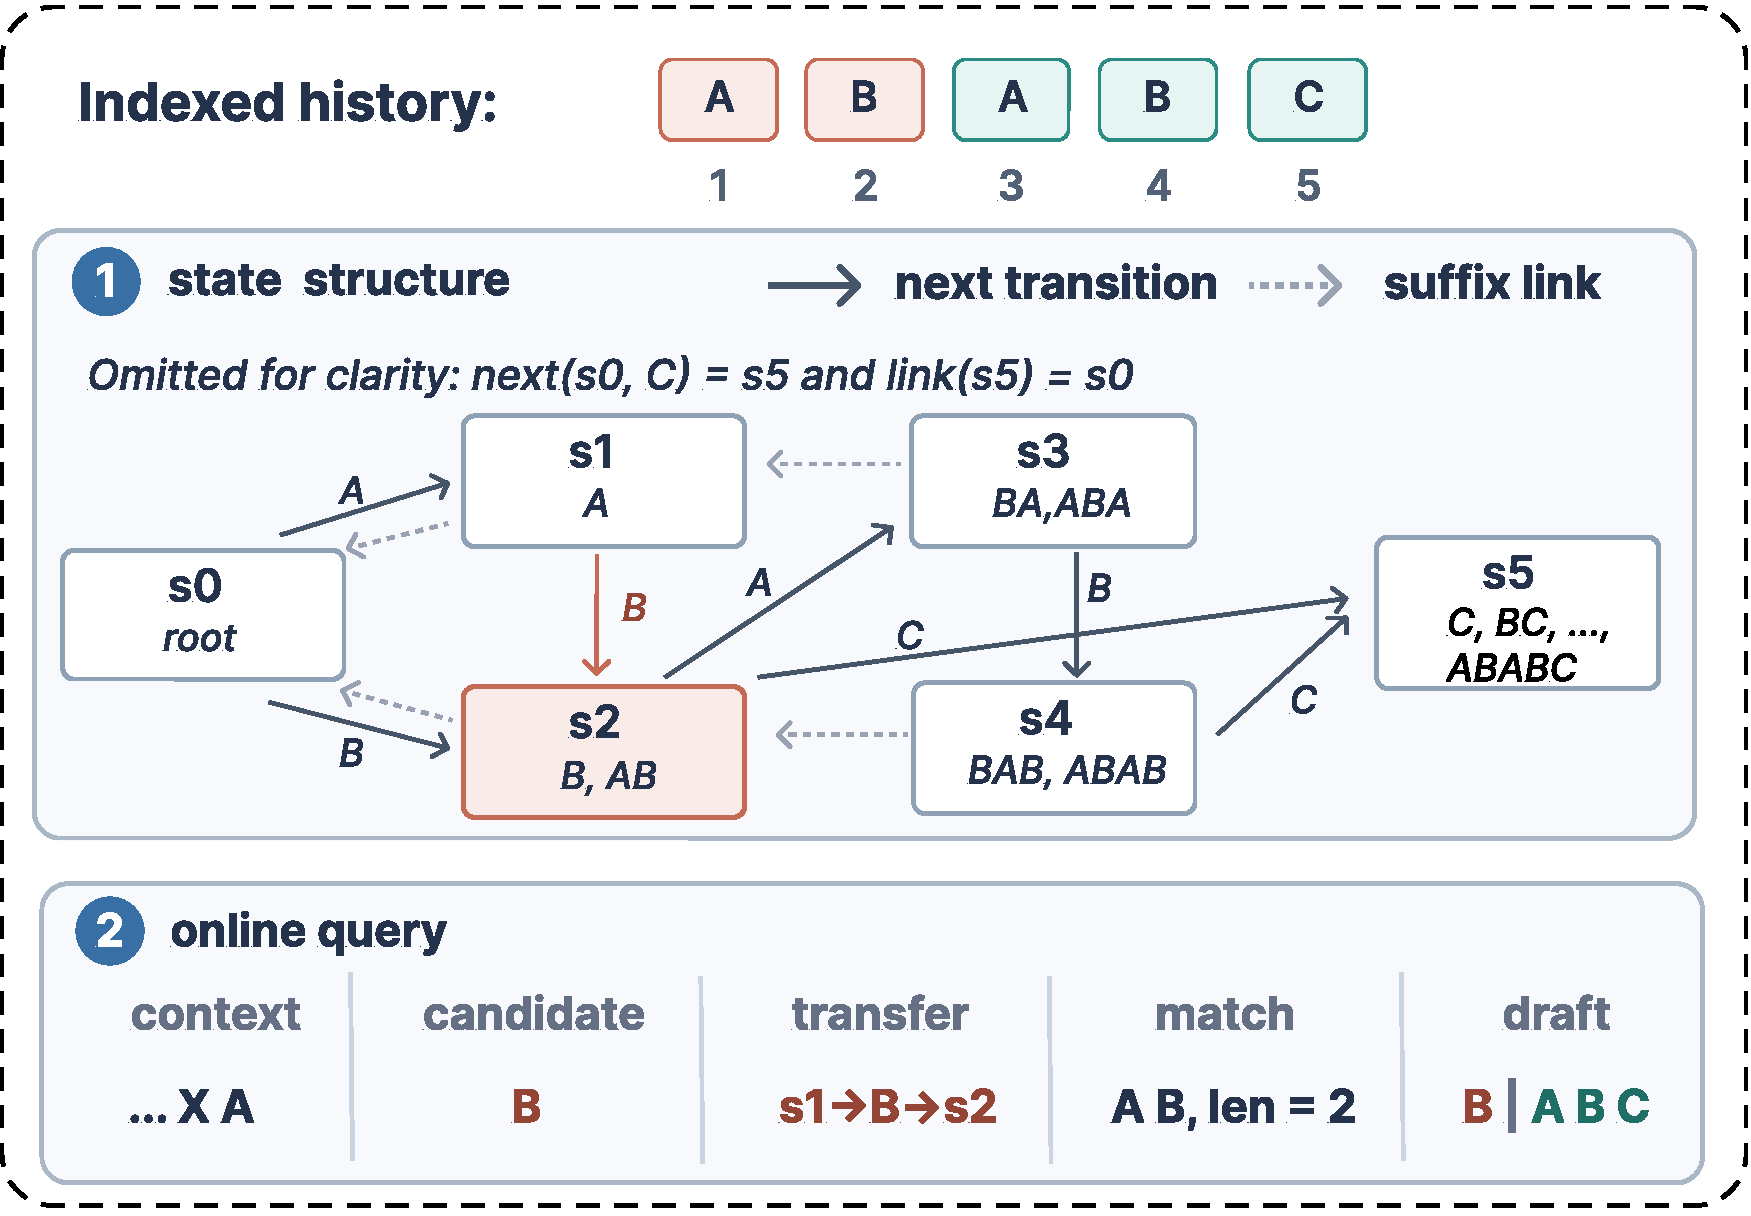
\includegraphics[width=1\columnwidth]{Figures/SAM.pdf}
    \caption{A suffix automaton for $T=\texttt{ABABC}$ and one online query. Black solid edges denote \texttt{next} transitions and gray dashed edges denote suffix links.}
    \label{fig:sam-example}
\end{figure}

\begin{figure}[t]
\begin{algbox}{Online SAM Extension}
	\footnotesize
	\label{alg:sam-build}
	\textbf{function} Extend\\
	\algindent \textbf{Input:} SAM $S$, token $z$, last state $last$, position $i$\\
	\algindent $cur \leftarrow \mathrm{NewState}()$\\
	\algindent $S[cur].\mathrm{len} \leftarrow S[last].\mathrm{len}+1$;
	$S[cur].\mathrm{minEnd} \leftarrow i$\\
	\algindent $p \leftarrow last$\\
	\algindent \textbf{while} $p \ne \bot$ and $z \notin S[p].\mathrm{next}$ \textbf{do}\\
	\algindenttwo $S[p].\mathrm{next}[z] \leftarrow cur$;
	$p \leftarrow S[p].\mathrm{link}$\\
	\algindent \textbf{end while}\\
	\algindent \textbf{if} $p=\bot$ \textbf{then}\\
	\algindenttwo $S[cur].\mathrm{link} \leftarrow S.\mathrm{root}$\\
	\algindent \textbf{else}\\
	\algindenttwo $q \leftarrow S[p].\mathrm{next}[z]$\\
	\algindenttwo \textbf{if} $S[p].\mathrm{len}+1=S[q].\mathrm{len}$ \textbf{then}\\
	\algindentthree $S[cur].\mathrm{link} \leftarrow q$\\
	\algindenttwo \textbf{else}\\
	\algindentthree $clone \leftarrow \mathrm{copy}(q)$;
	$S[clone].\mathrm{len} \leftarrow S[p].\mathrm{len}+1$\\
	\algindentthree \textbf{while} $p \ne \bot$ and $S[p].\mathrm{next}[z]=q$ \textbf{do}\\
	\algindentfour $S[p].\mathrm{next}[z] \leftarrow clone$;
	$p \leftarrow S[p].\mathrm{link}$\\
	\algindentthree \textbf{end while}\\
	\algindentthree $S[q].\mathrm{link},S[cur].\mathrm{link} \leftarrow clone$\\
	\algindenttwo \textbf{end if}\\
	\algindent \textbf{end if}\\
	\algindent $last \leftarrow cur$\\
	\algindent \textbf{Output:} updated $S$ and $last$\\
	\textbf{end function}
\end{algbox}
\end{figure}

\subsection{SAM-Based Local Draft Retrieval}

Algorithm~\ref{alg:sam-query} summarizes the local retrieval and online update procedure. During decoding, the cursor $(s,\ell)$ denotes the longest suffix of the current context found in the history: $s$ is its SAM state and $\ell$ its actual length. Both are needed because one state can represent several lengths. Given a token $z$, \textsc{Transfer} updates the cursor to the longest suffix ending in $z$ that occurs in the indexed history. If the current state has no transition for $z$, it follows suffix links to shorter suffixes and tests $z$ again. In contrast, $last$ is the construction pointer maintained by \textsc{Extend}: it identifies the SAM state representing the complete indexed history and serves as the starting point when a new token is inserted.

To retrieve a draft, \textsc{Retrieve} passes $z$ and the current cursor to \textsc{Transfer}, storing the result in a temporary cursor $(q,m)$ so that the original cursor remains unchanged. It returns no draft if the resulting match length $m$ is below $\ell_{\min}$. Otherwise, $S[q].\mathrm{minEnd}$ locates a representative occurrence from which up to $K$ continuation tokens are read. The target model subsequently verifies the retrieved draft. After verification, \textsc{Commit} processes accepted tokens in order: each advances the cursor through \textsc{Transfer} before insertion through \textsc{Extend}, preventing self-match. The cycle is \emph{retrieve $\rightarrow$ verify $\rightarrow$ transfer $\rightarrow$ extend}.

\begin{figure}[t]
\begin{algbox}{Online SAM Retrieval and Update}
	\footnotesize
	\label{alg:sam-query}
	\textbf{function} Transfer\\
	\algindent \textbf{Input:} SAM $S$, token $z$, state $s$, matching length $\ell$\\
	\algindent \textbf{while} $s \ne S.\mathrm{root}$ and $z \notin S[s].\mathrm{next}$ \textbf{do}\\
	\algindenttwo $s \leftarrow S[s].\mathrm{link}$;
	$\ell \leftarrow S[s].\mathrm{len}$\\
	\algindent \textbf{end while}\\
	\algindent \textbf{if} $z \in S[s].\mathrm{next}$ \textbf{then}\\
	\algindenttwo $s \leftarrow S[s].\mathrm{next}[z]$;
	$\ell \leftarrow \ell+1$\\
	\algindent \textbf{else}\\
	\algindenttwo $s \leftarrow S.\mathrm{root}$; $\ell \leftarrow 0$\\
	\algindent \textbf{end if}\\
	\algindent \textbf{Output:} next state $s$, next matching length $\ell$\\
	\textbf{end function}\\[2pt]
	\textbf{function} Retrieve\\
	\algindent \textbf{Input:} SAM $S$, history $T$, cursor $(s,\ell)$, candidate $z$\\
	\algindent \textbf{Parameters:} draft length $K$, threshold $\ell_{\min}$\\
	\algindent $(q,m) \leftarrow \mathrm{Transfer}(S,z,s,\ell)$\\
	\algindent \textbf{if} $m<\ell_{\min}$ \textbf{then return} $\varnothing,m$\\
	\algindent \textbf{while} $S[q].\mathrm{link} \ne S.\mathrm{root}$ and
	$K>|T|-S[q].\mathrm{minEnd}$ \textbf{do}\\
	\algindenttwo $q \leftarrow S[q].\mathrm{link}$\\
	\algindent \textbf{end while}\\
	\algindent $p \leftarrow S[q].\mathrm{minEnd}$\\
	\algindent $d \leftarrow [z] \,\Vert\, T[p+1:p+K-1]$\\
	\algindent Pad or truncate $d$ to length $K$\\
	\algindent \textbf{Output:} draft $d$, matching length $m$\\
	\textbf{end function}\\[2pt]
	\textbf{function} Commit\\
	\algindent \textbf{Input:} $S,T,(s,\ell),last$, accepted tokens $a_{1:u}$\\
	\algindent \textbf{for} $a \in a_{1:u}$ \textbf{do}\\
	\algindenttwo $(s,\ell) \leftarrow \mathrm{Transfer}(S,a,s,\ell)$\\
	\algindenttwo $(S,last) \leftarrow \mathrm{Extend}(S,a,last,|T|+1)$; $T \leftarrow T\Vert[a]$\\
	\algindent \textbf{end for}\\
	\algindent \textbf{Output:} updated $S,T,(s,\ell),last$\\
	\textbf{end function}
\end{algbox}
\end{figure}

\begin{figure*}[t]
    \centering
    
\includegraphics[width=0.98\textwidth]{"Figures/global index version 2.pdf"}
    \caption{Organization and pruning of the role-aware global index. Queries select a role, back off from longer to shorter anchors, and draft from the latest span associated with the matched anchor.}
    \label{fig:global-span-index}
\end{figure*}

\subsection{Role-Aware Global Index}

To reuse continuations across samples, MAReuse-D maintains a role-aware global index implemented as a hash-based span index. Figure~\ref{fig:global-span-index} illustrates its organization and optional pruning process. The index is organized as $G[r][L][a] \rightarrow \mathcal{L}$, where $r$ is an agent role, $L\in\{8,12,24\}$ is the anchor length, $a$ is an exact token anchor, and $\mathcal{L}$ is a bounded list of continuation entries. Each entry stores a tuple $(u,b,e)$ pointing to an eligible continuation $H_u[b:e]$ in source history $u$, with inclusive start $b$ and exclusive end $e$. This representation stores only a source identifier and two offsets rather than duplicating continuation tokens. When the same anchor is observed again, the new entry is added to the list, which is kept at a fixed maximum size.

At lookup, the current role selects its partition and the index tries longer anchors first. For a matched anchor, MAReuse-D ranks the entries in its list using lightweight evidence such as past hit count, recency, and available continuation length, and returns the selected referenced span subject to the draft budget for $L$. The index also supports TTL-based cold-anchor pruning as an optional memory-control mechanism: singleton anchors that survive for a configured number of completed samples without being hit can be removed, while few-shot anchors and multi-entry lists are retained. Unless otherwise specified, our main experiments use the unpruned index to isolate the effect of cross-sample reuse from memory-reduction heuristics.

The index is initially empty and persists across completed samples. After each sample finishes, its newly generated continuations are processed together and added to the index in a batch. This avoids repeated global-index updates during decoding and improves construction efficiency.

\subsection{Collaborative Decoding Procedure}

Algorithm~\ref{alg:collab-decoding} composes the preceding components. At each step, MAReuse-D first calls local \textsc{Retrieve} from Algorithm~\ref{alg:sam-query}; a match is valid only if it contains at least $\ell_{\min}$ exact tokens. Otherwise, it queries the role-aware global index using the longest available exact anchor. If neither linear source succeeds, it falls back to a logits-cache tree~\citep{DBLP:conf/acl/LuoWZZZ0X25}. Every selected draft is verified by the target model.

%The distinction between proposal and commitment is central: a retrieval hit only proposes tokens for verification. Only posterior-accepted tokens are appended to the generated history and committed to the sample-scoped SAM; their continuation entries are added to the global index after the sample completes. The logits cache is updated separately with top-$k$ target-model predictions from retained verified positions, which may include candidates that are not selected as output tokens. This update schedule supports three complementary forms of reuse. The local SAM captures cross-agent text overlap within the current input, the global index retrieves role-consistent continuations from completed inputs, and the logits cache reuses target-model candidate distributions as a role-agnostic fallback when no reliable exact match is available.

\begin{algbox}{Collaborative Decoding with Linear and Tree Drafts}
\label{alg:collab-decoding}
\textbf{function} DecodeWithReuse\\
\algindent \textbf{Input:} target model $M$, local SAM $S_{\mathrm{loc}}$, role-aware global index $G$, logits cache $C$, agent role $r$\\
\algindent \textbf{while} stopping condition is not met \textbf{do}\\
	\algindenttwo $d \leftarrow$ local SAM draft from $S_{\mathrm{loc}}$\\
\algindenttwo \textbf{if} $d$ is empty or its exact match is shorter than $\ell_{\min}$ \textbf{then}\\
\algindenttwo\algindent $d \leftarrow$ role-aware global draft from $G[r]$\\
\algindenttwo \textbf{end if}\\
\algindenttwo \textbf{if} $d$ is still empty (no configured exact anchor matches) \textbf{then}\\
\algindenttwo\algindent $d \leftarrow$ logits-cache tree draft from $C$\\
\algindenttwo \textbf{end if}\\
\algindenttwo Verify $d$ with the target model using linear or tree attention metadata\\
	\algindenttwo Let $(a_1,\ldots,a_u)$ be the tokens accepted by posterior verification\\
	\algindenttwo Commit $(a_1,\ldots,a_u)$ to $S_{\mathrm{loc}}$ by \textsc{Transfer} then \textsc{Extend}, in order\\
	\algindenttwo Update $C$ with the verified tokens and top-$k$ logits\\
\algindent \textbf{end while}\\
\algindent After the sample completes, insert role-separated accepted continuations into $G$\\
\textbf{end function}
\end{algbox}

\subsection{Memory Scope and Scaling}

\textbf{MAReuse-P.} Consider a transformer with $N$ layers, $n_{\mathrm{kv}}$ key/value heads, head dimension $d_h$, and hidden width $d$. For each token, the standard KV cache contains $2Nn_{\mathrm{kv}}d_h$ elements, accounting for both keys and values at every layer. MAReuse-P additionally retains one $d$-element hidden state at the input to the filter block for each reusable token. Both the KV cache and the additional hidden state use bf16 precision in our experiments. Taking Llama-3.1-8B-Instruct as an example, $N=32$, $n_{\mathrm{kv}}=8$, $d_h=128$, and $d=4096$. Its KV cache therefore contains 65,536 bf16 elements, or 128 KiB, per token, whereas the additional hidden state contains 4,096 bf16 elements, or 8 KiB. The additional storage is thus 6.25\% of the KV-only footprint. Following the prompt decomposition in Equation~1 of the main paper, hidden states for fixed segments $a_i$ remain cached across samples, while those for dynamic segments $z_i$ are released after the corresponding sample completes.

\textbf{MAReuse-D.} Let $T$ denote the number of tokens generated in the current sample. The sample-local SAM contains $O(T)$ states and is released when the sample completes. Retaining the top-$k$ token ids and scores at verified positions requires $O(kT)$ space in the logits cache. The role-aware global index, in contrast, persists across samples and deliberately trades memory for retrieval time: once an exact anchor has been formed, hash-table lookup takes expected $O(1)$ time. Let $H$ denote the total number of history tokens retained from completed samples, $A$ the number of configured anchor lengths, $L_{\max}$ the maximum anchor length, and $C$ the maximum number of references stored for each anchor. Across all anchor lengths, at most $AH$ anchor occurrences are indexed. Storing their keys requires $O(AHL_{\max})$ space, and their bounded reference lists require $O(AHC)$ space. The resulting space complexity is therefore $O(AH(L_{\max}+C))$. In our five-agent workflow, the measured growth of the unpruned index is approximately 0.8 MB per completed sample. For memory-constrained settings, the optional TTL-based policy removes eligible cold entries, thereby further reducing memory usage.


\section{Experiment Details}

This section describes the experimental setting used for the main results, including the multi-agent workflow, prompt templates, runtime environment, baseline implementations, and evaluation metrics.

\subsection{Experimental Environment}

All experiments are run on a server equipped with an Intel(R) Xeon(R) Platinum 8470Q CPU and a single NVIDIA GeForce RTX 4090 GPU. Model inference uses bfloat16 (bf16) precision on the GPU, with the same runtime precision and serving configuration applied to all methods. The software stack is PyTorch 2.11.0 with the CUDA 13.0 runtime and Transformers 4.50.2. In Transformers, we set the decoding temperature to 0 and use greedy decoding unless otherwise stated. All latency and throughput measurements use batch size 1. We use CUDA synchronization before and after timing.

\subsection{Method Configurations}

We compare MAReuse against performance bounds and state-of-the-art reuse methods, and report the configuration used for each method. All methods are implemented in the same Hugging Face Transformers-based codebase and use the same model, prompts, stopping rules, answer extraction scripts, and maximum generation limits for a given benchmark.

\noindent\textbf{Performance bounds.}
\begin{itemize}
    \item \textbf{Full Prefill}: the standard multi-agent pipeline that recomputes every assembled prompt from scratch. This establishes the quality reference for prefill reuse methods.
    \item \textbf{Autoregressive}: the target model's standard greedy decoding without speculative drafts. This establishes the decoding-throughput reference.
\end{itemize}

\noindent\textbf{Prefill reuse methods.}
\begin{itemize}
    \item \textbf{CacheBlend}~\citep{DBLP:conf/eurosys/YaoLLRCZD0J25}: a selective recomputation method that reuses aligned KV caches and corrects tokens with large shallow-layer KV deviations. Following the common setting, we select the top 20\% reused tokens for recomputation.
    \item \textbf{EPIC}~\citep{DBLP:conf/icml/HuHWWHZFCS025}: a position-independent context caching method that recomputes a fixed prefix window in each chunk. We implement the LegoLink correction with chunk size 16.
    \item \textbf{RelayCaching}~\citep{DBLP:journals/corr/abs-2603-13289}: a decode-to-prefill KV reuse method that transfers KV caches produced during upstream decoding and rectifies them with profiled layer-range and sparse-token correction. We use the recommended hyperparameters from the paper.
    \item \textbf{KVCOMM}~\citep{ye2026kvcomm}: a multi-agent KV communication framework that estimates prefix-conditioned KV offsets through similarity retrieval from role-specific anchor pools. We follow the default configuration of the original method and use an anchor pool size of 20 per agent role.
    \item \textbf{MAReuse-P}: our method with only filter-layer corrected prefill reuse enabled. We use layer 6 for Llama-3.1-8B-Instruct and layer 7 for Qwen2.5-Coder-7B-Instruct. We use the same dataset-level ratio as the target cardinality for both the layer-1 initial selection and the filter-layer reselection; the identities of the selected tokens may change after filtering. Decoding remains standard autoregressive decoding, isolating the prefill component.
\end{itemize}

\noindent\textbf{Decoding reuse methods.}
\begin{itemize}
    \item \textbf{Token Recycling}~\citep{DBLP:conf/acl/LuoWZZZ0X25}: a training-free speculative decoding method that stores top-$k$ candidate tokens from prior decoding steps and retrieves a logits tree for tree-attention verification. Following the original paper, we use its fixed 81-node tree template.
    \item \textbf{SAM-Decoding}~\citep{DBLP:conf/acl/HuWZZLCZ25}: a suffix-automaton-based speculative decoding method that retrieves repeated suffix continuations as linear drafts. Following the original paper, we use its 61-token draft budget.
    \item \textbf{RACER}~\citep{zhang2026racer}: a retrieval-enhanced speculative decoding method that combines logits-tree candidates with Aho-Corasick matching. Following the original paper, we use a 61-token draft budget and an Aho-Corasick automaton budget of 10,000 nodes.
	\item \textbf{MAReuse-D}: our method with only collaborative speculative decoding enabled, with normal prefill to isolate decoding acceleration. Local reuse uses a dynamic suffix automaton with minimum match length 5 and draft length up to 40. Global reuse uses role-aware anchors of lengths $\{8,12,24\}$, stores eligible continuation references, addresses up to 256 tokens per reference, and uses draft caps of 64, 128, and 256 tokens, respectively. The main experiments use the unpruned global index; the pruning rule described in the method details is an optional memory-control mechanism. If retrieval fails, the logits-cache fallback uses the fixed 81-node tree during the first 50 evaluated samples. These samples are part of the reported evaluation rather than a discarded warm-up set. MAReuse-D records only target-model-verified selected paths from these causally observed samples, then freezes a specialized 61-node template for subsequent samples; reference answers, correctness labels, and future samples are not used for specialization.
\end{itemize}

For end-to-end evaluation, \textbf{MAReuse} enables both MAReuse-P and MAReuse-D. Prefill speedup is measured by time-to-first-token (TTFT), while decoding speed is reported as generated tokens per second and mean accepted tokens per verification step (MAT). All speculative methods use posterior verification by the same target model; draft tokens are never accepted solely because they were retrieved or cached. For a given benchmark, methods also share the same prompts, greedy target-model policy, stopping rule, maximum output length, and answer extraction. The reported configurations follow the default or recommended budgets of the original methods rather than a separate per-benchmark search on evaluation accuracy.

\subsection{Workflow}

We use a feed-forward directed acyclic graph (DAG) for each multi-agent workflow. Agents are ordered by their execution stage. Agent 1 receives only the user question, while each downstream Agent $i$ receives the user question together with the outputs of all upstream agents $\{1,\ldots,i-1\}$. For example, Agent 2 receives \placeholder{agent\_1\_current}, Agent 3 receives both \placeholder{agent\_1\_current} and \placeholder{agent\_2\_current}, and the final agent aggregates all available upstream outputs. This topology contains edges from every earlier agent to every later agent and no backward edges, so information flows once from earlier reasoning stages to later verification and decision stages. We do not use multi-round history in these experiments. Workflow width counts all LLM calls, including the final decision-maker. A width-$m$ workflow uses the first $m-1$ specialist roles listed in the dataset-specific order below, followed by the corresponding top decision-maker; increasing width therefore adds one specialist without changing the feed-forward aggregation rule.

\subsection{Prompt Templates}

Our prompt templates follow the general design of KVCOMM~\citep{ye2026kvcomm}, including dataset-specific agent roles and placeholder-based context injection. We make small task-formatting and output-format adjustments for MAReuse, while keeping the overall multi-agent workflow comparable. Unless otherwise stated, \placeholder{user\_question} denotes the dataset input, \placeholder{agent\_i\_current} denotes the current-round output from Agent $i$, and \placeholder{condition\_i\_current} denotes tool or execution feedback associated with Agent $i$.

\paragraph{GSM8K}

For GSM8K, agents use complementary reasoning with shared code and execution feedback, and the final agent aggregates their outputs into a numeric answer.

\begin{promptbox}{Math Solver}
	You are a math expert. You will be given a math problem and hints from other agents. Give your own solving process step by step based on hints. The last line of your output contains only the final result without any units, for example: The answer is 140.
	
	You will be given some examples you may refer to.
	
	\placeholder{few\_shot\_example}
	
	The task is:
	
	\placeholder{user\_question}
\end{promptbox}

\begin{promptbox}{Mathematical Analyst}
	You are a mathematical analyst. You will be given a math problem, analysis and code from other agents. You need to first analyze the problem-solving process step by step, where the variables are represented by letters. Then you substitute the values into the analysis process to perform calculations and get the results. The last line of your output contains only the final result without any units, for example: The answer is 140.
	
	You will be given some examples you may refer to.
	
	\placeholder{few\_shot\_example}
	
	The task is:
	
	\placeholder{user\_question}
	
	At the same time, there are the following responses to the same question for your reference:
	
	Agent 1 as a Math Solver his answer to this question is:
	
	\placeholder{agent\_1\_current}
\end{promptbox}

\begin{promptbox}{Programming Expert}
	You are a programming expert. You will be given a math problem, analysis and code from other agents. Integrate step-by-step reasoning and Python code to solve math problems. Analyze the question and write functions to solve the problem. The function should not take any arguments and use the final result as the return value. The last line of code calls the function you wrote and assigns the return value to the \(answer\) variable. Use a Python code block to write your response. Do not include anything other than Python code blocks in your response.
	
	You will be given some examples you may refer to.
	
	\placeholder{few\_shot\_example}
	
	The task is:
	
	\placeholder{user\_question}
	
	At the same time, there are the following responses to the same question for your reference:
	
	Agent 1 as a Math Solver his answer to this question is:
	
	\placeholder{agent\_1\_current}
	
	Agent 2 as a Mathematical Analyst his answer to this question is:
	
	\placeholder{agent\_2\_current}
\end{promptbox}

\begin{promptbox}{Inspector}
	You are an Inspector. You will be given a math problem, analysis and code from other agents. Check whether the logic/calculation of the problem solving and analysis process is correct(if present). Check whether the code corresponds to the solution analysis(if present). Give your own solving process step by step based on hints. The last line of your output contains only the final result without any units, for example: The answer is 140.
	
	You will be given some examples you may refer to.
	
	The task is:
	
	\placeholder{user\_question}
	
	At the same time, there are the following responses to the same question for your reference:
	
	Agent 1 as a Math Solver his answer to this question is:
	
	\placeholder{agent\_1\_current}
	
	Agent 2 as a Mathematical Analyst his answer to this question is:
	
	\placeholder{agent\_2\_current}
	
	Agent 3 as a Programming Expert his answer to this question is:
	
	\placeholder{agent\_3\_current}
	
	the answer is \placeholder{condition\_3\_current}
\end{promptbox}

\begin{promptbox}{Top Decision-Maker}
	You are the top decision-maker. You will be given a math problem, analysis and code from other agents. Please find the most reliable answer based on the analysis and results of other agents. Give reasons for making decisions. The last line of your output contains only the final result without any units, for example: The answer is 140.
	
	The task is:
	
	\placeholder{user\_question}
	
	At the same time, the output of other agents is as follows:
	
	Agent 1, role is Math Solver, output is:
	
	\placeholder{agent\_1\_current}
	
	Agent 2, role is Mathematical Analyst, output is:
	
	\placeholder{agent\_2\_current}
	
	Agent 3, role is Programming Expert, output is:
	
	\placeholder{agent\_3\_current}
	
	the answer is \placeholder{condition\_3\_current}
	
	Agent 4, role is Inspector, output is:
	
	\placeholder{agent\_4\_current}
\end{promptbox}

\paragraph{MMLU}

For MMLU, agents combine entity extraction, Wikipedia-assisted reasoning, criticism, specialist reasoning, and final answer selection. The downstream agents receive the question together with upstream agent outputs through explicit placeholders.

\begin{promptbox}{Knowledgeable Expert}
	You are a knowledgeable expert in question answering.
	Please give at most six key entities that need to be searched in wikipedia to solve the problem.
	Key entities that need to be searched are included between two '@' when output, for example: @catfish effect@, @broken window effect@, @Shakespeare@.
	If there is no entity in the question that needs to be searched in Wikipedia, you don't have to provide it.
	
	The task is: \placeholder{user\_question}
\end{promptbox}

\begin{promptbox}{Wiki Searcher}
	You will be given a question and a wikipedia overview of the key entities within it.
	Please refer to them step by step to give your answer.
	And point out potential issues in other agent's analysis.
	
	The task is: \placeholder{user\_question}
	
	The key entities of the problem are explained in Wikipedia as follows: \placeholder{condition\_1\_current}
	
	At the same time, the outputs of other agents are as follows:
	
	Agent 1, role is Knowledgeable Expert, output is:
	
	\placeholder{agent\_1\_current}
\end{promptbox}

\begin{promptbox}{Critic}
	You are an excellent critic.
	Please point out potential issues in other agent's analysis point by point.
	
	The task is: \placeholder{user\_question}
	
	At the same time, the outputs of other agents are as follows:
	
	Agent 1, role is Knowledgeable Expert, output is:
	
	\placeholder{agent\_1\_current}
	
	Agent 2, role is Wiki Searcher, output is:
	
	\placeholder{agent\_2\_current}
\end{promptbox}

\begin{promptbox}{Mathematician}
	You are a mathematician who is good at math games, arithmetic calculation, and long-term planning.
	
	The task is: \placeholder{user\_question}
	
	At the same time, the outputs of other agents are as follows:
	
	Agent 1, role is Knowledgeable Expert, output is:
	
	\placeholder{agent\_1\_current}
	
	Agent 2, role is Wiki Searcher, output is:
	
	\placeholder{agent\_2\_current}
	
	Agent 3, role is Critic, output is:
	
	\placeholder{agent\_3\_current}
\end{promptbox}

\begin{promptbox}{MMLU Top Decision-Maker}
	You are the top decision-maker and are good at analyzing and summarizing other people's opinions, finding errors and giving final answers.
	
	You will receive a question followed by four possible answers labeled A, B, C, and D. Only one answer is correct.
	Choose the correct option based on the analysis and recommendations provided by the output of other agents.
	Your response must be exactly one of the letters A, B, C, or D, with no additional characters or text.
	
	The task is: \placeholder{user\_question}
	
	At the same time, the output of other agents is as follows:
	
	Agent 1, role is Knowledgeable Expert, output is:
	
	\placeholder{agent\_1\_current}
	
	Agent 2, role is Wiki Searcher, output is:
	
	\placeholder{agent\_2\_current}
	
	Agent 3, role is Critic, output is:
	
	\placeholder{agent\_3\_current}
	
	Agent 4, role is Mathematician, output is:
	
	\placeholder{agent\_4\_current}
\end{promptbox}

\paragraph{HumanEval}

For HumanEval, agents collaborate on code generation and debugging. Downstream agents receive upstream design notes, implementations, and internal-test feedback through explicit placeholders.

\begin{promptbox}{Project Manager}
	You are a project manager. You will be given a function signature and its docstring by the user. You are responsible for overseeing the overall structure of the code, ensuring that the code is structured to complete the task Implement code concisely and correctly without pursuing over-engineering. You need to suggest optimal design patterns to ensure that the code follows best practices for maintainability and flexibility. You can specify the overall design of the code, including the classes that need to be defined(maybe none) and the functions used (maybe only one function). I hope your reply will be more concise. Preferably within fifty words. Don't list too many points.
	
	The task is:
	
	\placeholder{user\_question}
\end{promptbox}

\begin{promptbox}{Algorithm Designer}
	You are an algorithm designer. You will be given a function signature and its docstring by the user. You need to specify the specific design of the algorithm, including the classes that may be defined and the functions used. You need to generate the detailed documentation, including explanations of the algorithm, usage instructions, and API references. When the implementation logic is complex, you can give the pseudocode logic of the main algorithm. I hope your reply will be more concise. Preferably within fifty words. Don't list too many points.
	
	\placeholder{few\_shot\_examples}
	
	The task is:
	
	\placeholder{user\_question}
	
	At the same time, the outputs and feedbacks of other agents are as follows:
	
	Agent 1 as a Project Manager provides the following info:
	
	\placeholder{agent\_1\_current}
\end{promptbox}

\begin{promptbox}{Programming Expert}
	You are a programming expert. You will be given a function signature and its docstring by the user. You may be able to get the output results of other agents. They may have passed internal tests, but they may not be completely correct. Write your full implementation (restate the function signature). Use a Python code block to write your response. Do not include anything other than Python code blocks in your response. Do not change function names and input variable types in tasks.
	
	The task is:
	
	\placeholder{user\_question}
	
	At the same time, the outputs and feedbacks of other agents are as follows:
	
	Agent 1 as a Project Manager provides the following info:
	
	\placeholder{agent\_1\_current}
	
	Agent 2 as an Algorithm Designer provides the following info:
	
	\placeholder{agent\_2\_current}
\end{promptbox}

\begin{promptbox}{Test Analyst}
	You are a test analyst. You will be given a function signature and its docstring by the user. You need to provide problems in the current code or solution based on the test data and possible test feedback in the question. You need to provide additional special use cases, boundary conditions, etc. that should be paid attention to when writing code. You can point out any potential errors in the code. I hope your reply will be more concise. Preferably within fifty words. Don't list too many points.
	
	The task is:
	
	\placeholder{user\_question}
	
	At the same time, the outputs and feedbacks of other agents are as follows:
	
	Agent 1 as a Project Manager provides the following info:
	
	\placeholder{agent\_1\_current}
	
	Agent 2 as an Algorithm Designer provides the following info:
	
	\placeholder{agent\_2\_current}
	
	Agent 3 as a Programming Expert:
	
	The code written by the agent is:
	
	\placeholder{agent\_3\_current}
	
	Whether it passes internal testing?
	
	\placeholder{condition\_3\_current}
\end{promptbox}

\begin{promptbox}{HumanEval Top Decision-Maker}
	You are the top decision-maker and are good at analyzing and summarizing other people's opinions, finding errors and giving final answers. And you are an AI that only responds with only python code.
	
	You will be given a function signature and its docstring by the user. You may be given the overall code design, algorithm framework, code implementation or test problems. Write your full implementation (restate the function signature). If the prompt given to you contains code that passed internal testing, you can choose the most reliable reply. If there is no code that has passed internal testing in the prompt, you can change it yourself according to the prompt. Use a Python code block to write your response. Do not include anything other than Python code blocks in your response.
	
	The task is:
	
	\placeholder{user\_question}
	
	At the same time, the output of other agents is as follows:
	
	Agent 1 as a Project Manager provides the following info:
	
	\placeholder{agent\_1\_current}
	
	Agent 2 as an Algorithm Designer provides the following info:
	
	\placeholder{agent\_2\_current}
	
	Agent 3 as a Programming Expert:
	
	The code written by the agent is:
	
	\placeholder{agent\_3\_current}
	
	Whether it passes internal testing?
	
	\placeholder{condition\_3\_current}
	
	Agent 4 as a Test Analyst provides the following info:
	
	\placeholder{agent\_4\_current}
	
	Agent 5 as a Bug Fixer:
	
	The code written by the agent is:
	
	\placeholder{agent\_5\_current}
	
	Whether it passes internal testing?
	
	\placeholder{condition\_5\_current}
\end{promptbox}


\section{Additional Experiment Results}

\subsection{Filter-Layer Selection on Qwen Models}

The main paper selects the MAReuse-P filter layer through an offline sweep on the target model. To evaluate whether this selection principle generalizes beyond the Llama-based settings, we conduct the same sweep on HumanEval using two Qwen-family models: Qwen2.5-Coder-7B-Instruct, used in our main HumanEval experiments, and Qwen2.5-7B-Instruct, a general-purpose instruction model. For each candidate layer, we use the same 20\% correction budget and measure the overall deviation reduction defined in Equation~(5) of the main paper.

\begin{figure}[t]
\centering
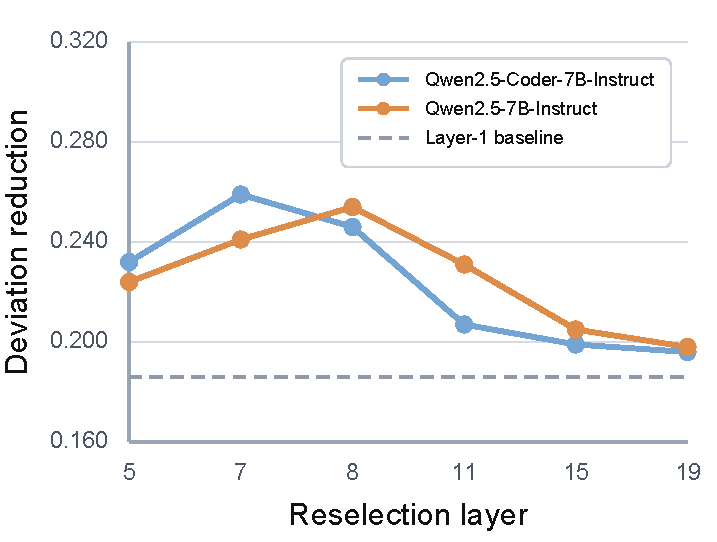
\includegraphics[width=\columnwidth]{Figures/supp_qwen_filter_layer.pdf}
\caption{Offline filter-layer sweep on Qwen-family instruction models using the HumanEval dataset. The curves report overall deviation reduction under different reselection layers, using layer-1 correction as the baseline.}
\label{fig:supp-qwen-filter-layer}
\end{figure}

Figure~\ref{fig:supp-qwen-filter-layer} reports the results using the same metric and visual convention as Figure~2 in the main paper. Both models exhibit a non-monotonic trend: intermediate layers achieve greater deviation reduction than layer-1 correction, whereas deeper layers leave fewer downstream layers to benefit from correction. This result supports selecting the filter layer through an offline model-specific sweep rather than fixing it solely based on model depth. Based on this sweep, we use layer 7 for Qwen2.5-Coder-7B-Instruct in the main HumanEval experiments and vary it only in the dedicated filter-layer ablation below.

\subsection{MMLU and HumanEval Filter-Layer Ablations}

We further report filter-layer ablations for MAReuse-P on MMLU and HumanEval. For MMLU, we evaluate 2--5 agent workflows with the same 25\% recomputation budget used in the main MMLU evaluation and vary only the filter layer, so the heatmap mainly reflects the placement of the re-selection operation. Figure~\ref{fig:supp-mmlu-filter-layer-ablation} shows that the average MMLU accuracy peaks at layer 6, consistent with the trend observed on GSM8K in the main paper. Wider MMLU workflows also degrade more noticeably at late layers, suggesting greater sensitivity to accumulated cache mismatch.

\begin{figure}[t]
\centering
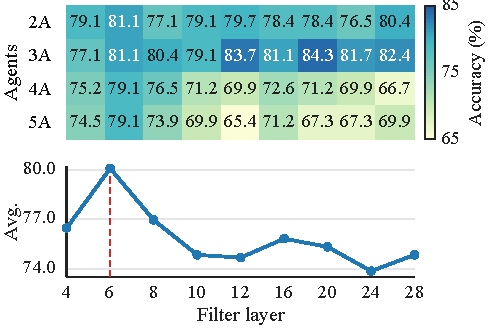
\includegraphics[width=\columnwidth]{Figures/supp_mmlu_filter_layer_ablation.pdf}
\caption{Filter-layer ablation on MMLU. The heatmap reports accuracy under different agent counts, and the lower curve shows the average accuracy across agent settings.}
\label{fig:supp-mmlu-filter-layer-ablation}
\end{figure}

We also sweep the filter layer on HumanEval under 2--5 agent workflows, using the same 20\% recomputation budget as the main evaluation. Figure~\ref{fig:supp-humaneval-filter-layer-ablation} shows a less pronounced but still non-monotonic pattern on HumanEval, with average Pass@1 peaking at layer 7 (86.96\%). Together, the two task-level sweeps support using layer 6 for Llama-3.1-8B-Instruct on MMLU and layer 7 for Qwen2.5-Coder-7B-Instruct on HumanEval, consistent with choosing the filter layer through an offline model- and task-specific sweep rather than fixing it by depth alone.

\begin{figure}[t]
\centering
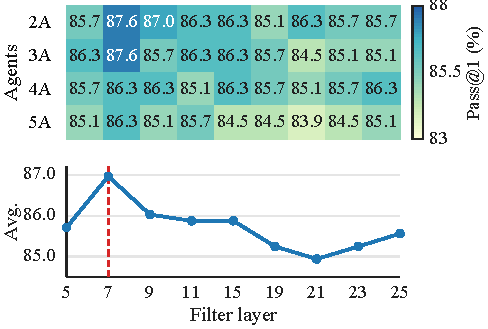
\includegraphics[width=\columnwidth]{Figures/supp_humaneval_filter_layer_ablation.pdf}
\caption{Filter-layer ablation on HumanEval. The heatmap reports Pass@1 under different agent counts, and the lower curve shows the average across agent settings.}
\label{fig:supp-humaneval-filter-layer-ablation}
\end{figure}



\subsection{Runtime Decomposition of MAReuse-D}

We further decompose MAReuse-D into model forward, draft generation, verification update, retrieval update, and logits update. This breakdown separates target-model computation from runtime state management introduced by collaborative drafting, and helps identify whether the remaining overhead comes from candidate construction or from maintaining reusable decoding state.

\begin{figure}[t]
	\centering
	
\includegraphics[width=\columnwidth]{"Figures/stage_runtime_breakdown.pdf"}
	\caption{Percentage of profiled generation time spent in different MAReuse-D runtime stages.}
	\label{fig:stage-runtime-breakdown}
\end{figure}

As shown in Figure~\ref{fig:stage-runtime-breakdown}, model forward accounts for 80.70\% of the runtime, indicating that performance is primarily determined by how many accepted tokens can be amortized over each target-model invocation. Verification update contributes another 11.56\%. During tree verification, the target-model forward produces KV states for all nodes in the candidate tree, including those on subsequently rejected branches. After the accepted path is selected, the KV cache must therefore be compacted: the original context and the KV states corresponding to the accepted nodes are retained, while rejected branches are removed and the retained states are repacked into a contiguous decoding history. This operation gathers and copies both key and value states at every transformer layer, introducing substantial memory movement and making verification update considerably more expensive than draft construction.

Retrieval update accounts for 5.76\%, reflecting an asymmetry between retrieval and maintenance: reading a continuation is inexpensive, whereas each accepted token must update suffix-automaton transitions and advance the collaborative retrieval state. Logits update contributes 1.26\%, as it only extracts and stores reusable top-$k$ successors from already computed logits. Consequently, draft generation itself requires only 0.72\% of the runtime. These results suggest that MAReuse-D introduces little candidate-construction overhead; its main optimization opportunities lie in increasing acceptance per target-model forward and reducing verification-update overhead.
\subsection{Accuracy Consistency of Decoding Baselines}

Although speculative decoding verifies draft tokens with the target model, it
may not be bitwise equivalent to autoregressive (AR) decoding on
finite-precision hardware. AR evaluates one token at a time, whereas
speculative decoding verifies multiple draft positions in parallel, sometimes
with a tree attention mask. The resulting differences in tensor shapes, GPU
kernels, and retained K/V states can slightly perturb the logits and accumulate
across steps. When the top two tokens have nearly identical logits, these
differences may change the \texttt{argmax} and cause the subsequent generation
paths to diverge. Our controlled analysis confirms that parallel
multi-token verification alone can cause this effect, while tree packing
introduces additional numerical variation. We therefore report the accuracy of
each decoding baseline separately.

\begin{table}[h]
\centering
\small
\setlength{\tabcolsep}{1.8pt}
\begin{tabular}{llccccc}
\thickhline
\textbf{Benchmark} & \textbf{Agents} & \textbf{AR} & \textbf{TR} & \textbf{RACER} & \textbf{SAMD} & \textbf{MAReuse-D} \\
\hline
\multirow{4}{*}{GSM8K}  & 2A & 84.67 & 84.22 & 83.61 & 83.92 & 83.16 \\
 & 3A & 84.37 & 83.76 & 82.55 & 84.52 & 84.07 \\
 & 4A & 84.37 & 83.31 & 84.52 & 84.22 & 83.76 \\
 & 5A & 84.07 & 84.52 & 83.76 & 84.22 & 83.76 \\
\hline
\multirow{4}{*}{MMLU} & 2A & 64.71 & 64.05 & 62.09 & 65.35 & 64.05 \\
 & 3A & 84.31 & 84.31 & 80.39 & 82.35 & 81.05 \\
 & 4A & 80.39 & 83.01 & 83.01 & 83.01 & 81.05 \\
 & 5A & 82.35 & 83.01 & 82.35 & 80.93 & 81.05 \\
\hline
\multirow{4}{*}{HumanEval} & 2A & 86.96 & 85.71 & 85.71 & 85.09 & 85.09 \\
 & 3A & 85.71 & 83.85 & 83.85 & 84.47 & 83.85 \\
 & 4A & 85.71 & 84.47 & 84.47 & 84.47 & 84.47 \\
 & 5A & 85.71 & 84.47 & 85.71 & 83.85 & 85.09 \\
\thickhline
\end{tabular}
\caption{Accuracy comparison of decoding baselines. AR denotes standard autoregressive decoding. TR denotes Token Recycling.}
\label{tab:decoding-accuracy-consistency}
\end{table}

Table~\ref{tab:decoding-accuracy-consistency} shows that the accuracy differences
between AR and speculative decoding remain within a few percentage points.
These differences reflect finite-precision decoding differences rather than
draft tokens bypassing target-model verification. MAReuse-D remains within the
empirical range of the other speculative baselines while providing higher
decoding throughput.

\subsection{Consolidated MMLU 2-Agent Results}

\begin{center}
\centering
\small
\setlength{\tabcolsep}{10pt}
\begin{tabular}{llc}
\thickhline
\textbf{Experiment} & \textbf{Method / setting} & \textbf{Acc.} \\
\hline
\multirow{6}{*}{Prefill}
 & Full Prefill + AR & 64.71 \\
 & CacheBlend + AR & 79.08 \\
 & EPIC + AR & 66.66 \\
 & RelayCaching + AR & 76.47 \\
 & KVCOMM + AR & 64.71 \\
 & MAReuse-P + AR & 81.70 \\
\hline
\multirow{5}{*}{Decoding}
 & Autoregressive & 64.71 \\
 & Token Recycling & 64.05 \\
 & RACER & 62.09 \\
 & SAM-Decoding & 65.35 \\
 & MAReuse-D & 64.05 \\
\hline
Combined & MAReuse-P + MAReuse-D & 81.05 \\
\hline
\multirow{5}{*}{Filter layer}
 & Layer 4 & 79.09 \\
 & Layer 8 & 77.12 \\
 & Layer 12 & 79.74 \\
 & Layer 20 & 78.43 \\
 & Layer 28 & 80.39 \\
\thickhline
\end{tabular}
\captionof{table}{Consolidated MMLU accuracy (\%) for the 2-agent workflow. AR denotes autoregressive decoding.}
\label{tab:mmlu-2a-consolidated}
\end{center}

Table~\ref{tab:mmlu-2a-consolidated} consolidates the MMLU 2-agent accuracy results from the main paper and supplementary material. The large gap between full prefill and MAReuse-P should not be interpreted as evidence that approximate KV reuse generally improves model reasoning. Instead, it reflects an instability specific to the 2-agent topology, in which the final decision-maker receives only the entity-oriented output of a single upstream expert and therefore has limited option-level evidence. A diagnostic analysis of the predicted labels shows that Full Prefill + AR selects option A in 54.25\% of the questions, whereas A constitutes only 31.37\% of the ground-truth labels. MAReuse-D retains a similar A-selection rate of 53.59\%, consistent with speculative verification preserving the target model's original decision behavior. In contrast, MAReuse-P changes the intermediate states used for final decision generation and reduces the A-selection rate to 38.56\%, bringing the predicted label distribution closer to the ground-truth distribution. Its accuracy gain in this setting is therefore associated primarily with mitigating a workflow-specific option-selection bias, rather than with an intrinsic quality advantage of approximate reuse. The consistently higher results across multiple filter layers further indicate that this effect is not confined to a single layer choice, while the combined pipeline largely inherits the improved prefill behavior. EPIC has less flexibility to address this instability because it applies a fixed correction pattern, whereas KVCOMM falls back to the full-prefill behavior when cache matching fails and consequently inherits much of the same 2-agent behavior.

\bibliography{aaai2027}

\end{document}
